% ============================================================
% Section 3: Method
% ============================================================

\section{Method}
\label{sec:method}

% ---------------------------------------------------------
\subsection{Task Definition}
\label{sec:method:task}
% ---------------------------------------------------------

Given a raster P\&ID image $I$, we aim to extract the process graph
$G = (V, E)$, where:
\begin{itemize}[noitemsep, topsep=2pt]
    \item $V$ is a set of detected physical components, each with a
          bounding box $(x_1, y_1, x_2, y_2)$ and a class label from
          \{\textit{valve, pump, instrumentation, general, tank, arrow,
          inlet/outlet}\};
    \item $E$ is a set of pipe or signal connections between components,
          each labelled \textit{solid} or \textit{non-solid}.
\end{itemize}

\noindent\textbf{Connector collapsing.}
\label{sec:method:collapse}
Raw P\&ID annotations contain \textit{connector} nodes
(${\approx}8\times8$~px routing waypoints) and \textit{crossing} nodes
(pipe-over-pipe non-connections) that together account for 50--65\% of
all annotated nodes but carry no physical meaning.
We collapse connector chains into direct component-to-component edges
(majority-vote edge label along each chain) and remove crossing nodes
before training and evaluation.
This reduces the problem to industrially meaningful connectivity and
aligns with the evaluation protocol of~\cite{sturmer2025}.

% ---------------------------------------------------------
\subsection{Topology-Preserving Synthetic Generation}
\label{sec:method:generation}
% ---------------------------------------------------------

\begin{figure*}[t]
    \centering
    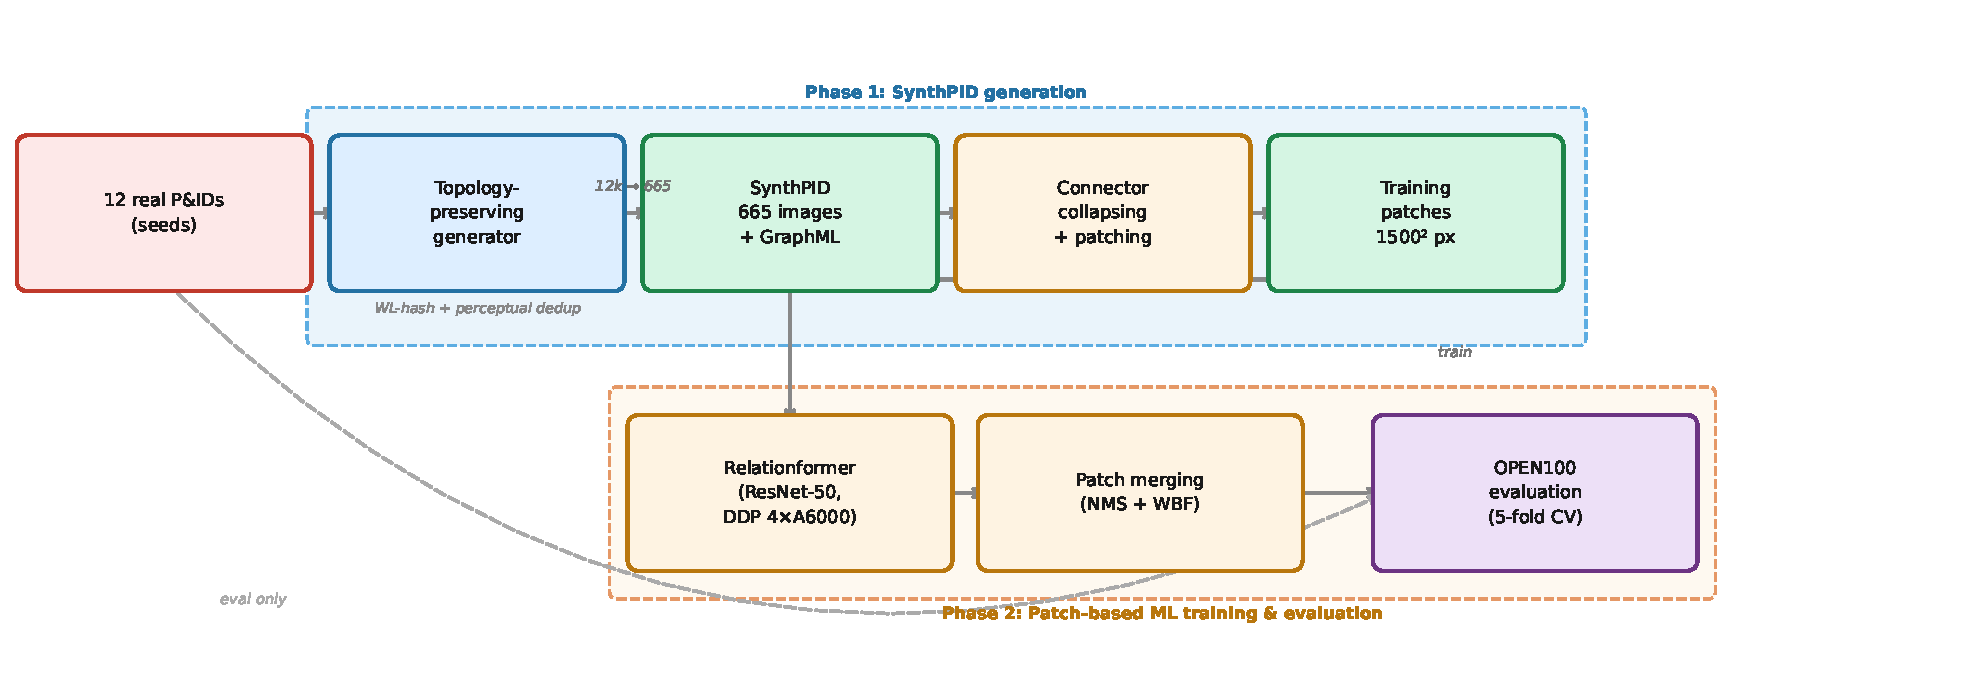
\includegraphics[width=\linewidth]{figures/pipeline_overview.pdf}
    \caption{
        \textbf{Overview of our approach.}
        Starting from 12 real-world P\&ID seeds, our topology-preserving
        generator produces \ours{} --- 665 structurally diverse
        synthetic P\&IDs with full graph-level annotations.
        A Relationformer trained on \ours{} with no real training data
        processes each P\&ID via overlapping patches and merges the
        resulting predictions into a complete process graph, which is
        evaluated on unseen real OPEN100 P\&IDs.
    }
    \label{fig:pipeline}
\end{figure*}

Figure~\ref{fig:pipeline} illustrates the full pipeline.
The key departure from prior work is \emph{how} synthetic data is created.

\noindent\textbf{Template-based generation (prior work).}
Existing synthetic P\&ID datasets~\cite{paliwal2021,sturmer2025} place
symbol templates at random positions on a blank canvas and connect them
according to a simplified grid layout.
The resulting graphs have unrealistic degree distributions and spatial
structure inconsistent with real process plants.
This mismatch explains the poor transfer reported
in~\cite{sturmer2025} (${\sim}33\%$ edge mAP with synth-only training).

\noindent\textbf{Topology-preserving generation (ours).}
We seed the generator from real P\&IDs.
Each generation step proceeds as follows:
\begin{enumerate}[noitemsep, topsep=2pt, leftmargin=1.3em]
    \item \textbf{Seed extraction.} Apply connector collapsing to a real
          P\&ID to obtain the physical component graph
          $G_s = (V_s, E_s)$.
    \item \textbf{Structural perturbation.} Spatially perturb node
          positions within topological constraints; substitute symbols
          within the same class for visual diversity.
    \item \textbf{Edge routing.} Re-route pipe connections via
          Manhattan routing while preserving graph adjacency.
    \item \textbf{Rendering.} Render the perturbed layout to PNG
          alongside a synchronised GraphML annotation.
    \item \textbf{Quality control.}
          Reject the candidate if its Weisfeiler-Lehman
          hash~\cite{shervashidze2011} matches any previously accepted
          graph (structural deduplication), or if its perceptual
          hash~\cite{phash} matches any prior image (visual
          deduplication).
\end{enumerate}

From ${\sim}12{,}000$ generation attempts seeded from 12 real P\&IDs,
we accept \textbf{665 structurally and visually diverse} synthetic
P\&IDs, constituting \ours{}.

\noindent\textbf{Visual and structural domain gap.}
Figure~\ref{fig:dataset_comparison} illustrates the visual gap between
real and synthetic P\&IDs: real OPEN100 diagrams have white backgrounds,
black line art, and professional title blocks, while SynthPID images have
a grey background and slightly different rendering style.
Despite this visual gap, the two corpora share the same symbol vocabulary
and, crucially, realistic pipe topology — which Figure~\ref{fig:graph_stats}
confirms quantitatively.
Our main result (63.8\% edge mAP) demonstrates that topology alignment
is sufficient for effective synthetic-to-real transfer even in the
presence of this visual gap.

\begin{figure}[h]
    \centering
    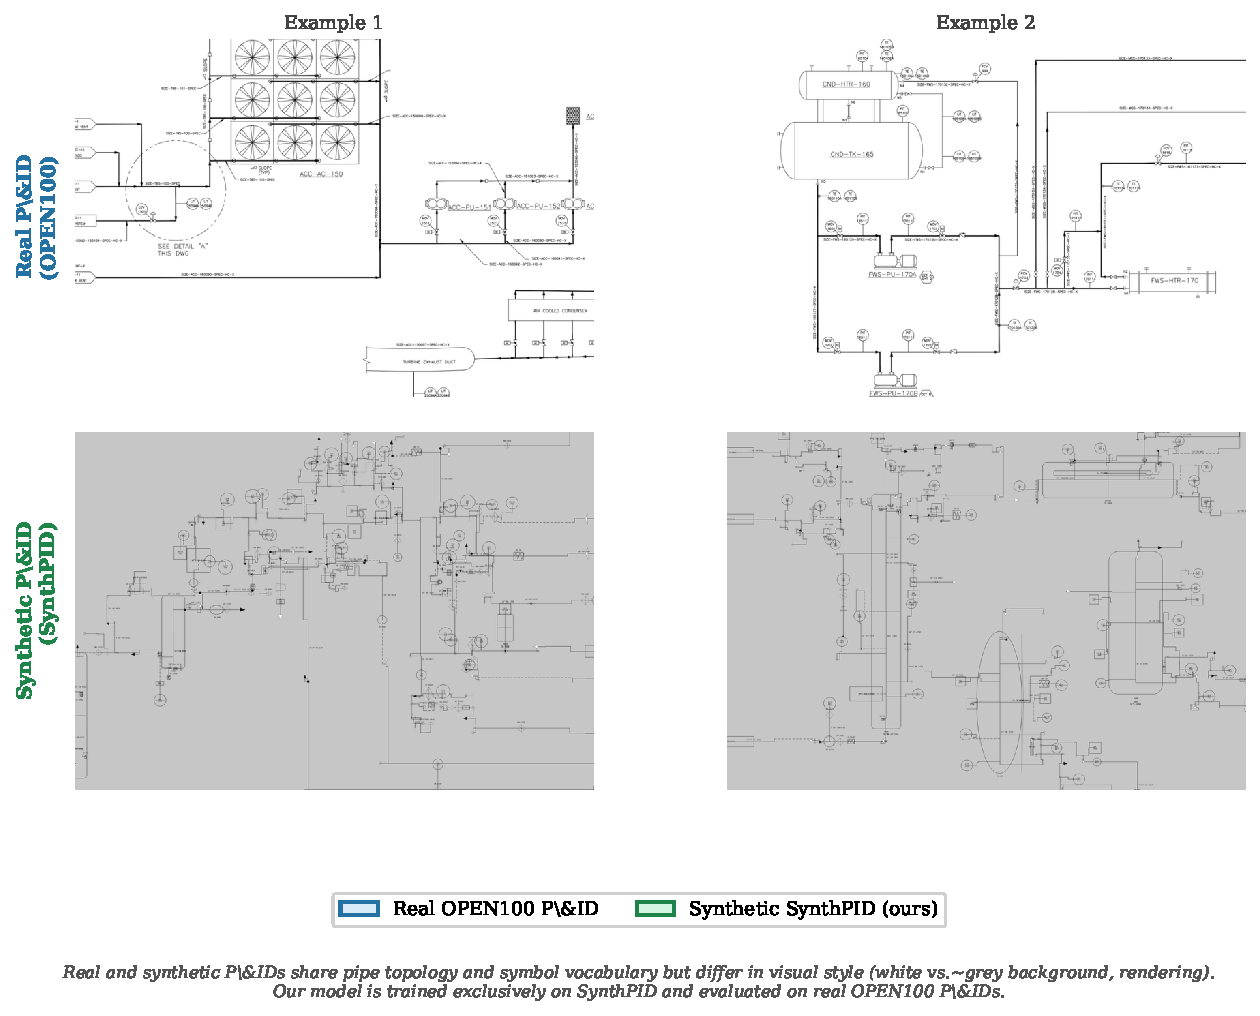
\includegraphics[width=\linewidth]{figures/dataset_comparison.pdf}
    \caption{
        \textbf{The synthetic-to-real domain gap.}
        Real OPEN100 P\&IDs (top, white background) vs.\
        SynthPID (bottom, grey background).
        Both share the same symbol classes and pipe topology, but differ
        substantially in visual appearance.
        Our model is trained exclusively on SynthPID and evaluated on
        the real OPEN100 images.
    }
    \label{fig:dataset_comparison}
\end{figure}

\noindent\textbf{Why topology preservation matters.}
Figure~\ref{fig:graph_stats} compares the degree distributions and edge
densities of \ours{} versus OPEN100 versus template-based data.
Our topology-preserving generation closely matches the real distribution,
while template-based data exhibits artificial regularity.
We attribute the +30~pp performance gap between the two strategies
(${\sim}33\%$ vs.\ 63.8\% edge mAP) directly to this structural
alignment.

\begin{figure}[h]
    \centering
    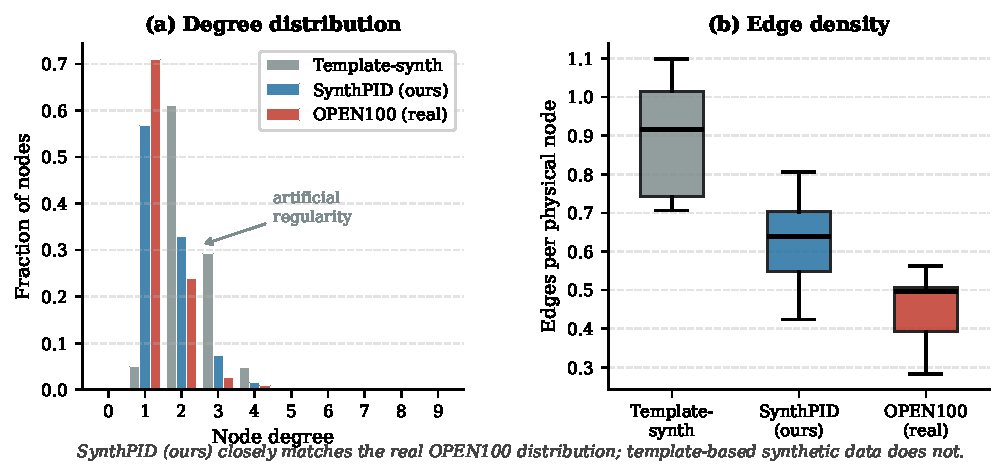
\includegraphics[width=\linewidth]{figures/graph_statistics.pdf}
    \caption{
        Degree distribution and edge density comparison.
        \ours{} (ours) closely matches OPEN100 (real).
        Template-based synthetic data exhibits artificial regularity
        inconsistent with real plant graphs.
    }
    \label{fig:graph_stats}
\end{figure}

% ---------------------------------------------------------
\subsection{Patch-Based Processing}
\label{sec:method:patching}
% ---------------------------------------------------------

P\&ID images are high-resolution (${\sim}7000\times4500$~px) and contain
symbols as small as $8\times8$~pixels.
Processing the full image at the resolutions required by a DETR-based
detector (800~px long side) reduces symbols to sub-pixel scale, making
box regression intractable.
Following~\cite{sturmer2025}, we split each full-resolution P\&ID into
overlapping patches of size $1500\times1500$~px with a stride of 750~px,
giving each symbol a representative footprint of 50--200~px within its
patch --- well within the operating range of Deformable~DETR.

\noindent\textbf{Patch creation.}
Each P\&ID is resized to $4500\times7000$~px before patching.
Where a pipe or connection exits a patch boundary, a \emph{border node}
is inserted at the intersection point to enable stitching across patches.

\noindent\textbf{Prediction merging.}
After per-patch inference, predictions are merged into a full-plan graph:
\begin{enumerate}[noitemsep, topsep=2pt, leftmargin=1.3em]
    \item Confidence scores are attenuated for boxes near patch borders,
          as these may represent partially-cropped symbols.
    \item Duplicate detections across overlapping patches are suppressed
          via Non-Maximum Suppression (NMS), then refined by
          Weighted Box Fusion (WBF)~\cite{solovyev2021}.
    \item Predicted edges are merged: border nodes from adjacent patches
          are matched and edges across patch boundaries are reconnected.
    \item Self-loops and isolated nodes are removed.
\end{enumerate}

Both \ours{} (training) and OPEN100 (evaluation) are processed through
this identical patching pipeline, ensuring consistent scale between
training and evaluation.

% ---------------------------------------------------------
\subsection{Graph Extraction Model}
\label{sec:method:model}
% ---------------------------------------------------------

We adopt Relationformer~\cite{shit2022} as our graph extraction backbone,
following~\cite{sturmer2025} to hold architecture constant across all
experimental configurations so that performance differences are
attributable to training data.
Relationformer enhances Deformable~DETR~\cite{zhu2021} with a shared
\emph{relation token} that is combined pairwise with object queries to
predict edges.
Its output is a set of $N$ detected nodes (bounding box + class) and
an edge adjacency prediction over all $\binom{N}{2}$ pairs per patch.

We configure the model for P\&ID extraction: 7~node classes
(Table~\ref{tab:classes}), 2~edge classes (solid, non-solid), and 401
object queries per patch (matching~\cite{sturmer2025}).
The edge loss weight is set to $\lambda_\text{edge}=5.0$ to prioritise
connectivity learning.

\begin{table}[h]
\centering
\caption{Node and edge vocabulary used for training and evaluation.}
\label{tab:classes}
\small
\begin{tabular}{ll}
\toprule
\textbf{Node classes (7)} & \textbf{Edge classes (2)} \\
\midrule
valve, pump, instrumentation & solid \\
general, tank, arrow, inlet/outlet & non-solid \\
\bottomrule
\end{tabular}
\end{table}

% ---------------------------------------------------------
\subsection{Evaluation Metric}
\label{sec:method:metric}
% ---------------------------------------------------------

We implement the edge mAP metric of~\cite{sturmer2025} (Algorithm~A1)
to ensure direct numerical comparability.
Hungarian matching~\cite{kuhn1955} aligns predicted nodes to
ground-truth nodes by bounding-box gIoU on the full stitched plan.
A predicted edge is a true positive only if both matched endpoints are
correct and the edge class agrees.
Average Precision is computed via the precision-recall curve and averaged
over the two edge classes.
We also report \textit{node mAP@0.5~IoU} per class on the stitched plan.
